\section{CƠ SỞ LÝ THUYẾT}
\subsection{Tìm hiểu về Restaurant Industry}

\subsubsection{Nhà hàng ăn uống cao cấp (Fine dining restaurant)}
\subsubsubsection{Tổng quan}
Fine dining được định nghĩa là trải nghiệm nhà hàng tinh tế, thường đắt đỏ và đặc biệt hơn so với nhà hàng thông thường. Đặc điểm bao gồm sử dụng khăn trải bàn trắng, dịch vụ bàn bởi nhân viên được đào tạo, và không gian sang trọng với vật liệu cao cấp. Lịch sử cho thấy fine dining bắt đầu vào những năm 1780 tại Paris, với các nhà hàng như Trois Frères và La Grande Taverne de Londres, và sau đó lan sang Hoa Kỳ với Delmonico's ở New York, nổi tiếng với hầm rượu 1.000 chai. Trong thời kìh hiện đại, fine dining tập trung vào sự sáng tạo và dịch vụ hoàn hảo.\\


\begin{figure}[H]
    \centering
    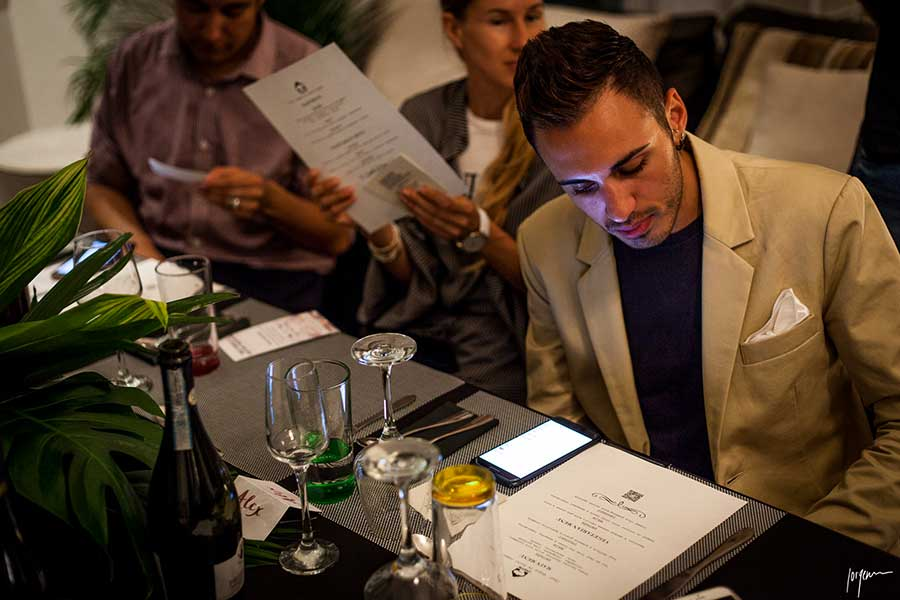
\includegraphics[width=15cm]{Images/fine-dining.jpg}
    \vspace{0.5cm}
    \caption{Nhà hàng fine dining. Nguồn: \href{https://chefin.com/blog/the-past-and-future-of-fine-dining/}{chefin.com}}
    \label{fig:my_label}
\end{figure}

Nhà hàng fine dining hoạt động dựa trên mô hình kinh doanh cân bằng giữa chi phí vận hành cao và giá bán cao cấp. Chi phí bao gồm nguyên liệu cao cấp, lao động có kỹ năng, và sự chú ý chi tiết trong cả chuẩn bị món ăn và dịch vụ. Doanh thu chủ yếu đến từ việc bán bữa ăn, với giá cao hơn nhiều so với nhà hàng ăn uống thông thường, phản ánh chất lượng và sự độc quyền của trải nghiệm. Ngoài ra, các chương trình rượu vang và đồ uống cũng đóng góp đáng kể vào doanh thu, cùng với các dịch vụ như tiệc riêng, catering, và bán hàng hóa. \\

Tuy nhiên, lợi nhuận trong fine dining là một thách thức do chi phí cố định và biến đổi cao. Chi phí cố định bao gồm tiền thuê ở vị trí đắc địa, trang trí cao cấp, và thiết bị, trong khi chi phí biến đổi bao gồm nguyên liệu đắt tiền và lao động cho đội ngũ được đào tạo bài bản. Thành công phụ thuộc vào việc duy trì tỷ lệ khách cao, khách hàng trung thành, và danh tiếng mạnh, có thể dẫn đến các giải thưởng như sao Michelin, từ đó thúc đẩy nhu cầu. \\

Fine dining hiện đại đã phát triển, nhấn mạnh vào sự sáng tạo và dịch vụ hoàn hảo. Sự kết hợp giữa chỗ ở sang trọng và ẩm thực cao cấp, như được tiên phong bởi César Ritz và Auguste Escoffier tại Grand Hotel of Monte Carlo, đã nâng tầm vị thế của fine dining.


\subsubsubsection{Sơ đồ tổ chức (Organization chart)}
Trong ngành công nghiệp nhà hàng, đặc biệt là nhà hàng ẩm thực cao cấp, sơ đồ tổ chức đóng vai trò quan trọng trong việc định hình cấu trúc, đảm bảo bộ máy hoạt động hiệu quả. Biểu đồ tổ chức giúp làm rõ mối quan hệ giữa các vị trí công việc, xác định ai báo cáo cho ai, và ai chịu trách nhiệm cho những nhiệm vụ cụ thể nào. Điều này đặc biệt quan trọng trong nhà hàng ẩm thực cao cấp, nơi mà chất lượng dịch vụ và sự hài lòng của khách hàng là yếu tố hàng đầu. \\
Nhà hàng ẩm thực cao cấp thường có cấu trúc tổ chức phức tạp và đa tầng, phản ánh nhu cầu cung cấp dịch vụ cá nhân hóa và sang trọng:

\begin{itemize}
    \item Quản trị viên: Vai trò này đảm bảo rằng nhà hàng tuân thủ các quy định pháp lý và hoạt động hành chính suôn sẻ. Họ xử lý thuế, làm việc với nhà cung cấp, và quản lý các vấn đề tài chính, tạo nền tảng cho hoạt động của nhà hàng.
    \item Quản lý: Là người giám sát tổng thể, đảm bảo rằng mọi bộ phận hoạt động hài hòa. Họ làm cầu nối giữa quản trị viên và các trưởng bộ phận, đảm bảo dịch vụ đạt tiêu chuẩn cao cấp.
    \item Quản lý nhà bếp: Vai trò này tập trung vào việc duy trì nguồn cung nguyên liệu chất lượng, làm việc chặt chẽ với đầu bếp trưởng để đảm bảo nhà bếp hoạt động hiệu quả.
    \item Đầu bếp trưởng: Là linh hồn của nhà hàng, chịu trách nhiệm cho tầm nhìn ẩm thực. Họ tạo ra thực đơn sáng tạo, phản ánh phong cách của nhà hàng, và giám sát toàn bộ hoạt động nhà bếp để đảm bảo chất lượng và sự nhất quán.
    \item Phó đầu bếp: Hỗ trợ đầu bếp trưởng, đảm bảo rằng mọi món ăn được chuẩn bị và trình bày đúng tiêu chuẩn, đặc biệt trong giờ cao điểm.
    \item Đầu bếp chuyên khoa: Mỗi station chef chịu trách nhiệm cho một lĩnh vực cụ thể, như món khai vị hoặc món chính, đảm bảo chuyên môn hóa và chất lượng cao.
    \item Đầu bếp, trợ lý: Là lực lượng hỗ trợ chính, thực hiện các nhiệm vụ hàng ngày như chuẩn bị nguyên liệu và nấu nướng, đảm bảo nhà bếp hoạt động trơn tru.
    \item Người rửa chén, nhân viên dọn dẹp hậu trường: Vai trò này rất quan trọng để duy trì vệ sinh, đảm bảo an toàn thực phẩm, và giữ cho nhà bếp luôn sẵn sàng.
    \item Trưởng phục vụ (Maitre d'): Là gương mặt đại diện của nhà hàng, đảm bảo khách hàng có trải nghiệm đầu tiên ấn tượng. Họ quản lý danh sách đặt chỗ và hướng dẫn khách, tạo nên bầu không khí chuyên nghiệp.
    \item Nhân viên phục vụ: Đảm bảo khách hàng được phục vụ chu đáo, từ việc lấy order đến phục vụ món ăn, góp phần vào trải nghiệm tổng thể.
    \item Chuyên viên rượu: Là chuyên gia về rượu, họ tư vấn cho khách hàng về các lựa chọn rượu phù hợp, nâng cao trải nghiệm ẩm thực, đặc biệt trong môi trường cao cấp.
    \item Nhân viên dọn dẹp tiền sảnh: Giữ khu vực ăn uống sạch sẽ và ngăn nắp, đảm bảo không gian sang trọng và thoải mái cho khách hàng.
    \item Trưởng bảo vệ: Quản lý an ninh, đảm bảo an toàn cho khách và tài sản, một vai trò quan trọng trong môi trường cao cấp.
    \item Bảo vệ, người đỗ xe: Cung cấp dịch vụ an ninh và đỗ xe, tạo ấn tượng chuyên nghiệp và sang trọng, đặc biệt cho khách hàng sử dụng dịch vụ đỗ xe.
\end{itemize}

\begin{table}[ht]
\centering
\resizebox{\textwidth}{!}{
    \begin{tabular}{| p{4cm} | p{11cm} | p{3cm} |}
    \hline
    \textbf{Vị trí} & \textbf{Chức năng} & \textbf{Báo cáo cho} \\
    \hline
    Quản trị viên (Administrator) & Xử lý thuế, nhà cung cấp, và các nhu cầu hành chính khác. Đảm bảo tuân thủ pháp lý và hoạt động hành chính suôn sẻ. & Không có (cấp cao nhất) \\
    \hline
    Quản lý (Manager) & Giám sát toàn bộ hoạt động của nhà hàng, bao gồm cả phần front-of-house và back-of-house. Đảm bảo dịch vụ chuyên nghiệp và khách hàng hài lòng. & Quản trị viên \\
    \hline
    Quản lý nhà bếp (Kitchen Manager) & Quản lý hàng tồn kho và mua sắm cho nhà bếp, đảm bảo nguyên liệu chất lượng cao. Làm việc chặt chẽ với đầu bếp trưởng. & Quản trị viên \\
    \hline
    Đầu bếp trưởng (Executive Chef) & Là người lãnh đạo culinaire, tạo thực đơn sáng tạo, giám sát hoạt động nhà bếp, đảm bảo chất lượng và sự nhất quán. & Quản lý nhà bếp \\
    \hline
    Phó đầu bếp (Sous-Chef) & Hỗ trợ đầu bếp trưởng, giám sát việc chuẩn bị và trình bày món ăn, đảm bảo tiêu chuẩn. & Đầu bếp trưởng \\
    \hline
    Đầu bếp chuyên khoa (Station Chef) & Chuyên trách một lĩnh vực cụ thể (khai vị, món chính, tráng miệng), xử lý chuẩn bị phức tạp, giám sát đầu bếp và trợ lý. & Phó đầu bếp \\
    \hline
    Đầu bếp, trợ lý (Cooks, Assistants) & Thực hiện nhiệm vụ được giao, bao gồm chuẩn bị nguyên liệu, nấu nướng, và trình bày món ăn. & Đầu bếp chuyên khoa \\
    \hline
    Người rửa chén, nhân viên dọn dẹp hậu trường (Dishwasher, Back of House Cleaners) & Giữ nhà bếp và thiết bị sạch sẽ, đảm bảo vệ sinh và an toàn thực phẩm. & Quản lý nhà bếp \\
    \hline
    Trưởng phục vụ (Maitre d') & Là gương mặt đầu tiên, hướng dẫn khách, quản lý danh sách đặt chỗ, đảm bảo dịch vụ xuất sắc. & Quản lý \\
    \hline
    Nhân viên phục vụ (Waiters) & Phục vụ khách, lấy order, phục vụ thức ăn và đồ uống, đảm bảo khách hài lòng. & Trưởng phục vụ \\
    \hline
    Chuyên viên rượu (Sommelier) & Là chuyên gia về rượu, tư vấn lựa chọn rượu phù hợp, nâng cao trải nghiệm ẩm thực. & Trưởng phục vụ \\
    \hline
    Nhân viên dọn dẹp tiền sảnh (Front-of-House Cleaning Staff) & Giữ khu vực ăn uống sạch sẽ và ngăn nắp, đảm bảo không gian thoải mái và sang trọng. & Trưởng phục vụ \\
    \hline
    Trưởng bảo vệ (Head of Security) & Quản lý an ninh, giám sát camera, bảo vệ, và người đỗ xe, đảm bảo an toàn cho khách và tài sản. & Quản lý \\
    \hline
    Bảo vệ, người đỗ xe (Guards, Valets) & Cung cấp dịch vụ an ninh và đỗ xe, tạo ấn tượng chuyên nghiệp và sang trọng. & Trưởng bảo vệ \\
    \hline
    \end{tabular}
}
\caption{Vị trí, chức năng và người quản lý trong một nhà hàng ăn uống cao cấp}
\end{table}

\clearpage

\begin{figure}[H]
    \centering
    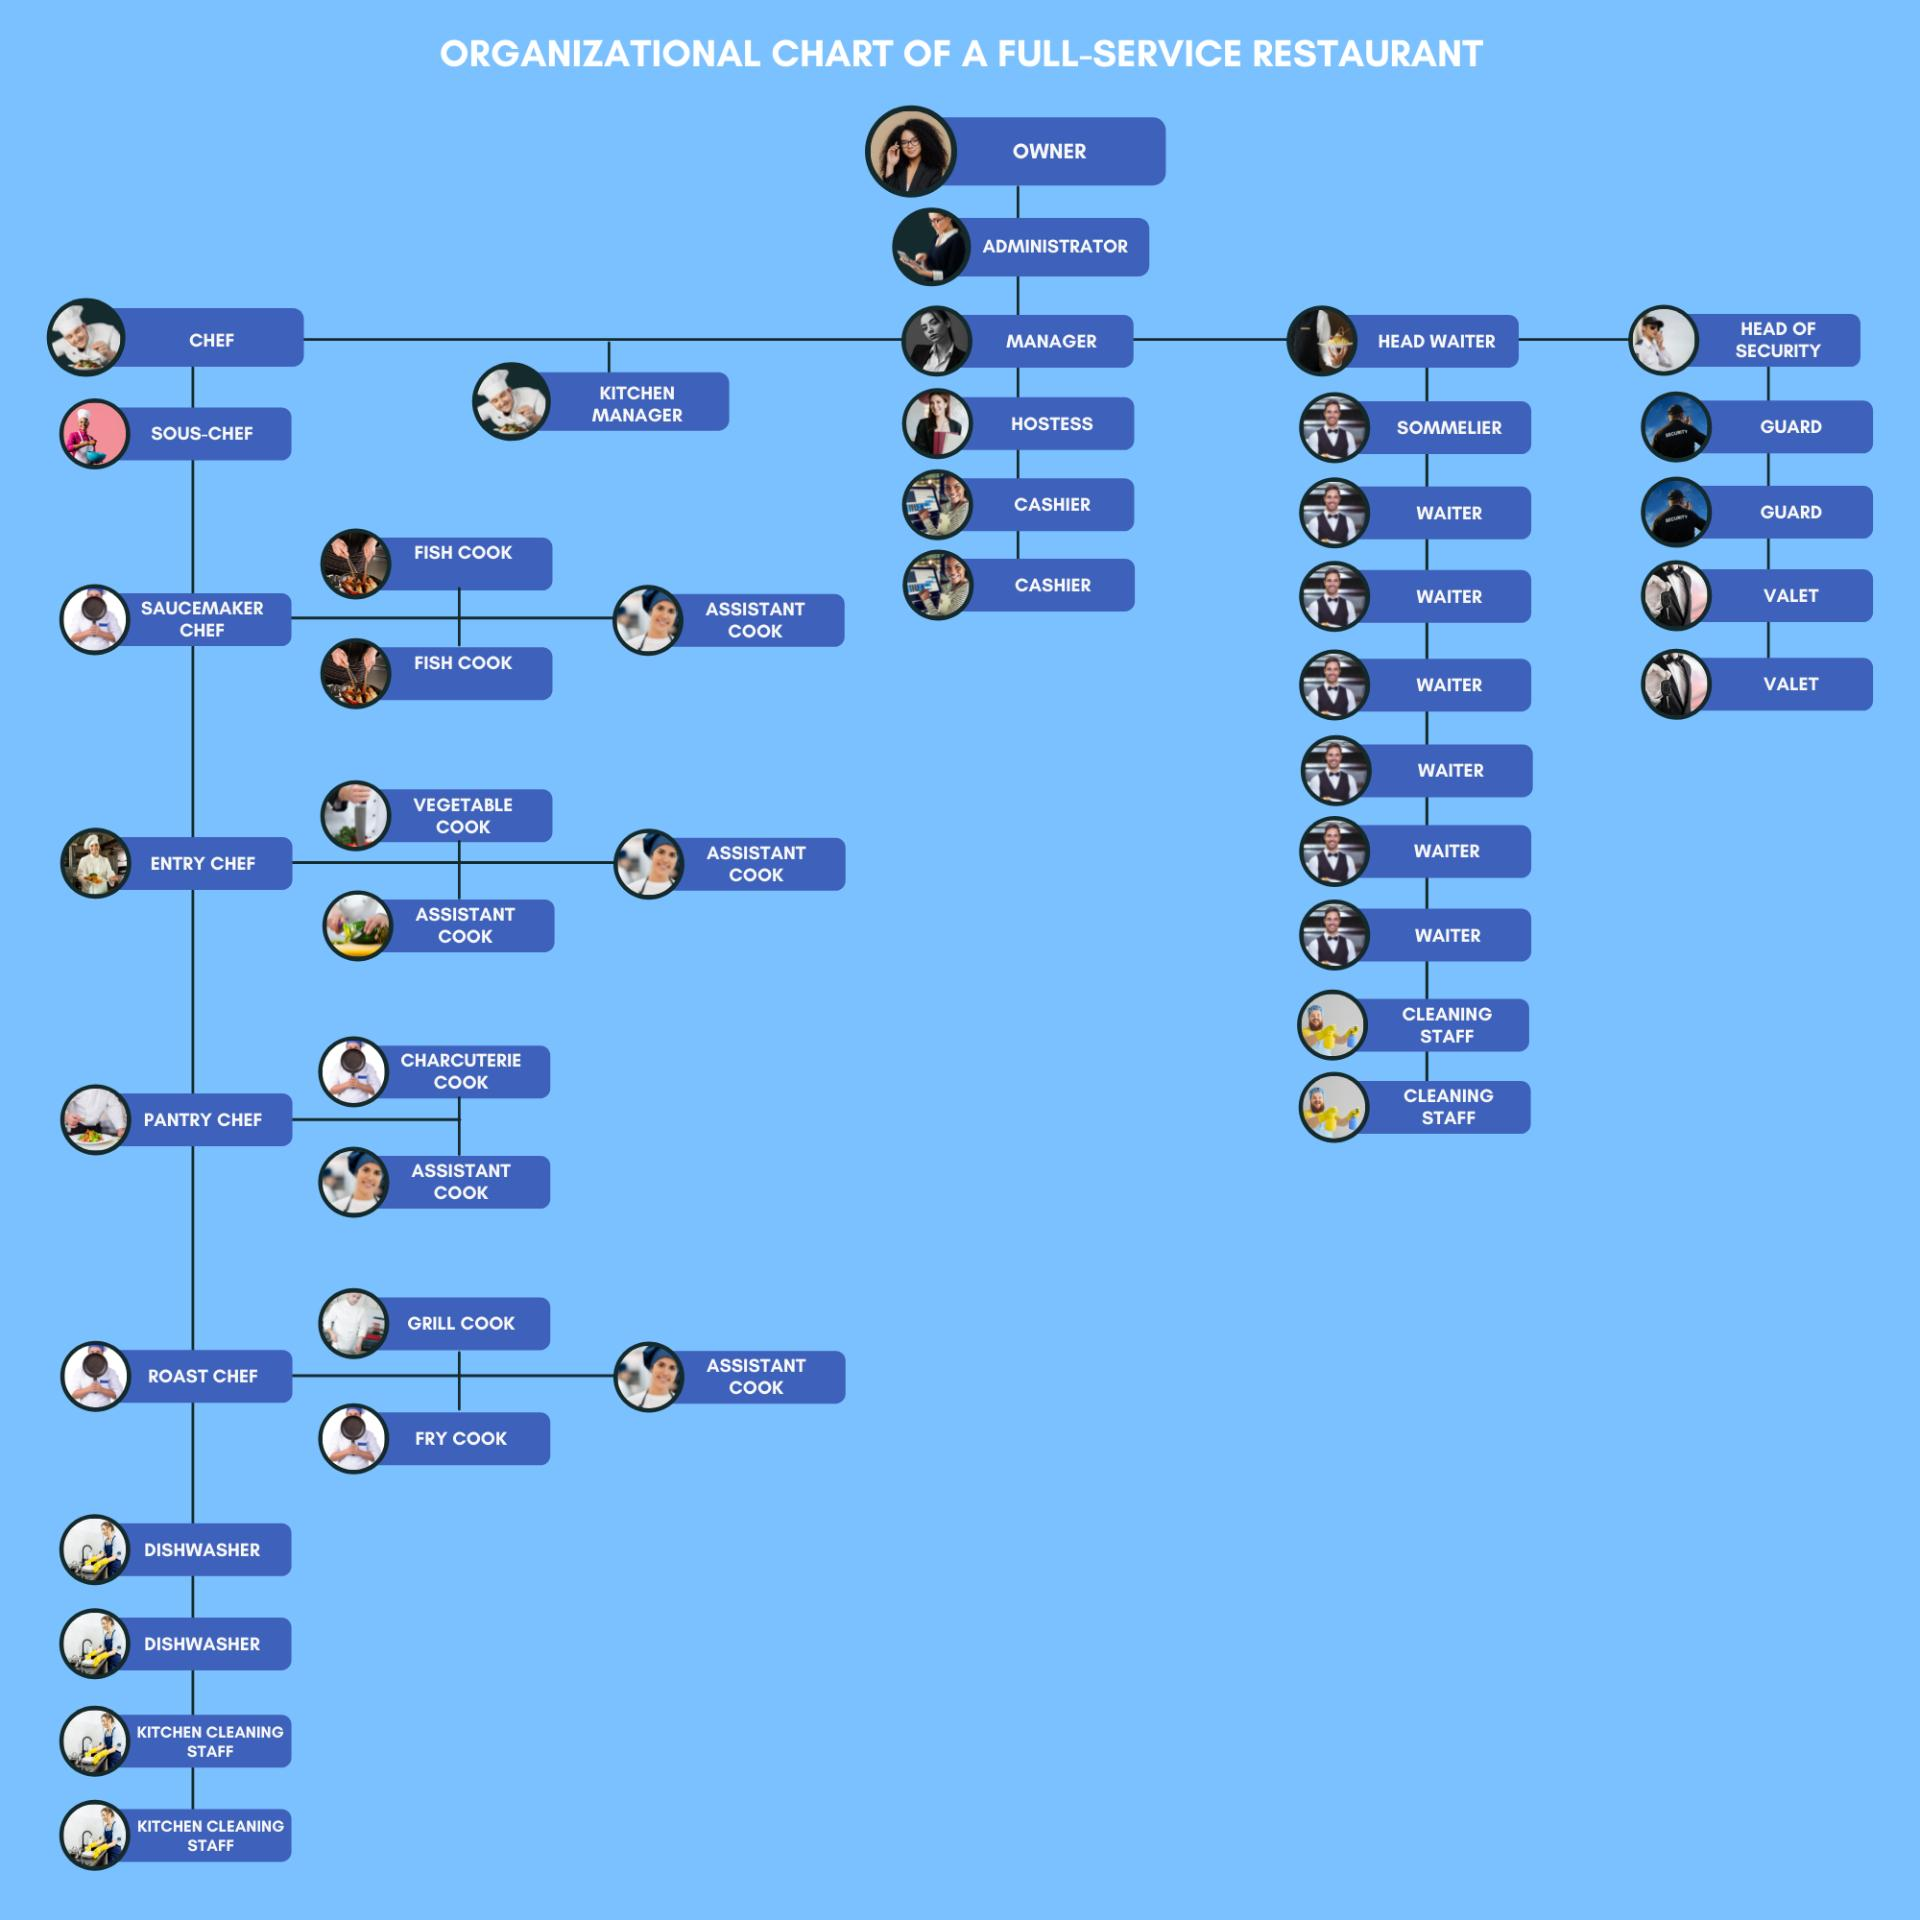
\includegraphics[width=15cm]{Images/finedining_orig_chart.jpg}
    \vspace{0.5cm}
    \caption{Sơ đồ tổ chức cho nhà hàng ăn uống cao cấp. Nguồn: waiterio.com}
\end{figure}

\subsubsection{Nhà hàng ăn uống phục vụ đồ ăn nhanh (Fast-food restaurant)}
\subsubsubsection{Tổng quan}
Nhà hàng thức ăn nhanh, còn được gọi là nhà hàng dịch vụ nhanh (QSR), là cơ sở cung cấp thức ăn được chuẩn bị và phục vụ nhanh chóng, thường trong vòng vài phút, với thực đơn hạn chế như bánh burger, khoai tây chiên, pizza và gà rán, phục vụ trong đồ dùng một lần. Khách hàng thường đặt hàng tại quầy hoặc qua cửa sổ giao hàng, và thức ăn được dự định để ăn tại chỗ hoặc mang đi. \\


\begin{figure}[H]
    \centering
    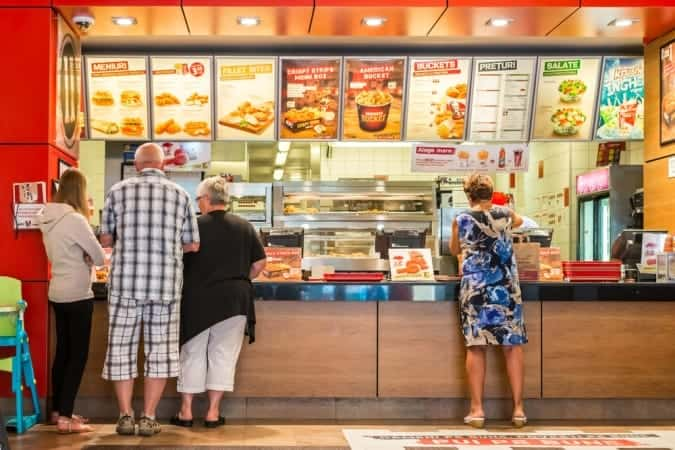
\includegraphics[width=15cm]{Images/fastfood.jpg}
    \vspace{0.5cm}
    \caption{Nhà hàng phụ vụ thức ăn nhanh. Nguồn: \href{https://foodtank.com/news/2015/08/world-health-organization-study-proves-need-for-regulation-of-fast-food/}{foodtank.com}}
\end{figure}

Mô hình kinh doanh của nhà hàng thức ăn nhanh tập trung vào khối lượng lớn và biên lợi nhuận thấp, với thực đơn chuẩn hóa và hệ thống franchise để đảm bảo sự đồng nhất và khả năng mở rộng. Họ nhắm đến thị trường bận rộn, sử dụng tiếp thị mạnh mẽ và nền tảng kỹ thuật số để tiếp cận khách hàng.

Nhà hàng thức ăn nhanh vận hành với các quy trình tinh giản sử dụng bếp dây chuyền để đảm bảo hiệu quả, với chuỗi cung ứng tập trung và công nghệ như hệ thống POS để tối ưu hóa hoạt động. Đào tạo nhân viên tập trung vào tốc độ và chính xác, với mô hình tự phục vụ giảm chi phí lao động.

\subsubsubsection{Sơ đồ tổ chức (Organization chart)}
Nhà hàng thức ăn nhanh thường có cấu trúc tổ chức đơn giản và phẳng, phản ánh nhu cầu cung cấp dịch vụ nhanh chóng và hiệu quả:
\begin{itemize}
    \item Quản lý điều hành: Giám sát toàn bộ hoạt động, bao gồm tuyển dụng và ngân sách.
    \item Quản lý ca: Giám sát nhân viên trong ca, xử lý khiếu nại khách hàng.
    \item Nhân viên thu ngân: Xử lý thanh toán và đơn hàng.
    \item Đầu bếp: Chuẩn bị thức ăn, đảm bảo chất lượng.
    \item Nhân viên vệ sinh: Giữ nhà hàng sạch sẽ, đặc biệt quan trọng trong môi trường cao áp lực.
\end{itemize}
\begin{table}[ht]
\centering
\resizebox{\textwidth}{!}{
    \begin{tabular}{| p{4cm} | p{11cm} | p{3cm} |}
    \hline
    \textbf{Vị trí} & \textbf{Chức năng} & \textbf{Báo cáo cho} \\
    \hline
    Quản lý điều hành (Executive Manager) & Giám sát toàn bộ hoạt động của nhà hàng, bao gồm tuyển dụng, sa thải, ngân sách, lương, lịch trình, hàng tồn kho, và mua sắm nguyên liệu. & Không có (cấp cao nhất) \\
    \hline
    Quản lý ca (Shift Manager) & Giám sát nhân viên trong ca làm việc, xử lý khiếu nại khách hàng, lập lịch, kiểm tra tiền thu ngân. & Quản lý điều hành \\
    \hline
    Nhân viên thu ngân (Cashier) & Xử lý đơn hàng và thanh toán của khách hàng. & Quản lý ca \\
    \hline
    Nhân viên ghi order (Order Taker) & Ghi đơn hàng, đặc biệt ở đường lái xe. & Quản lý ca \\
    \hline
    Nhân viên dịch vụ khách hàng (Customer Service Representative) & Hỗ trợ giải quyết các câu hỏi hoặc vấn đề của khách hàng. & Quản lý ca \\
    \hline
    Đầu bếp và nhân viên bếp (Cooks and Kitchen Staff) & Chuẩn bị thức ăn, bổ sung nguyên liệu, bảo trì thiết bị. & Quản lý ca \\
    \hline
    Nhân viên rửa chén (Dishwasher) & Duy trì vệ sinh nhà bếp. & Quản lý ca \\
    \hline
    Nhân viên bảo trì (Maintenance Staff) & Xử lý sửa chữa thiết bị. & Quản lý ca \\
    \hline
    Nhân viên vệ sinh (Cleaning Crew) & Giữ cho nhà hàng sạch sẽ. & Quản lý ca \\
    \hline
    \end{tabular}
}
\caption{Vị trí, chức năng và người quản lý trong một nhà hàng phục vụ đồ ăn nhanh}
\end{table}

\begin{figure}[H]
    \centering
    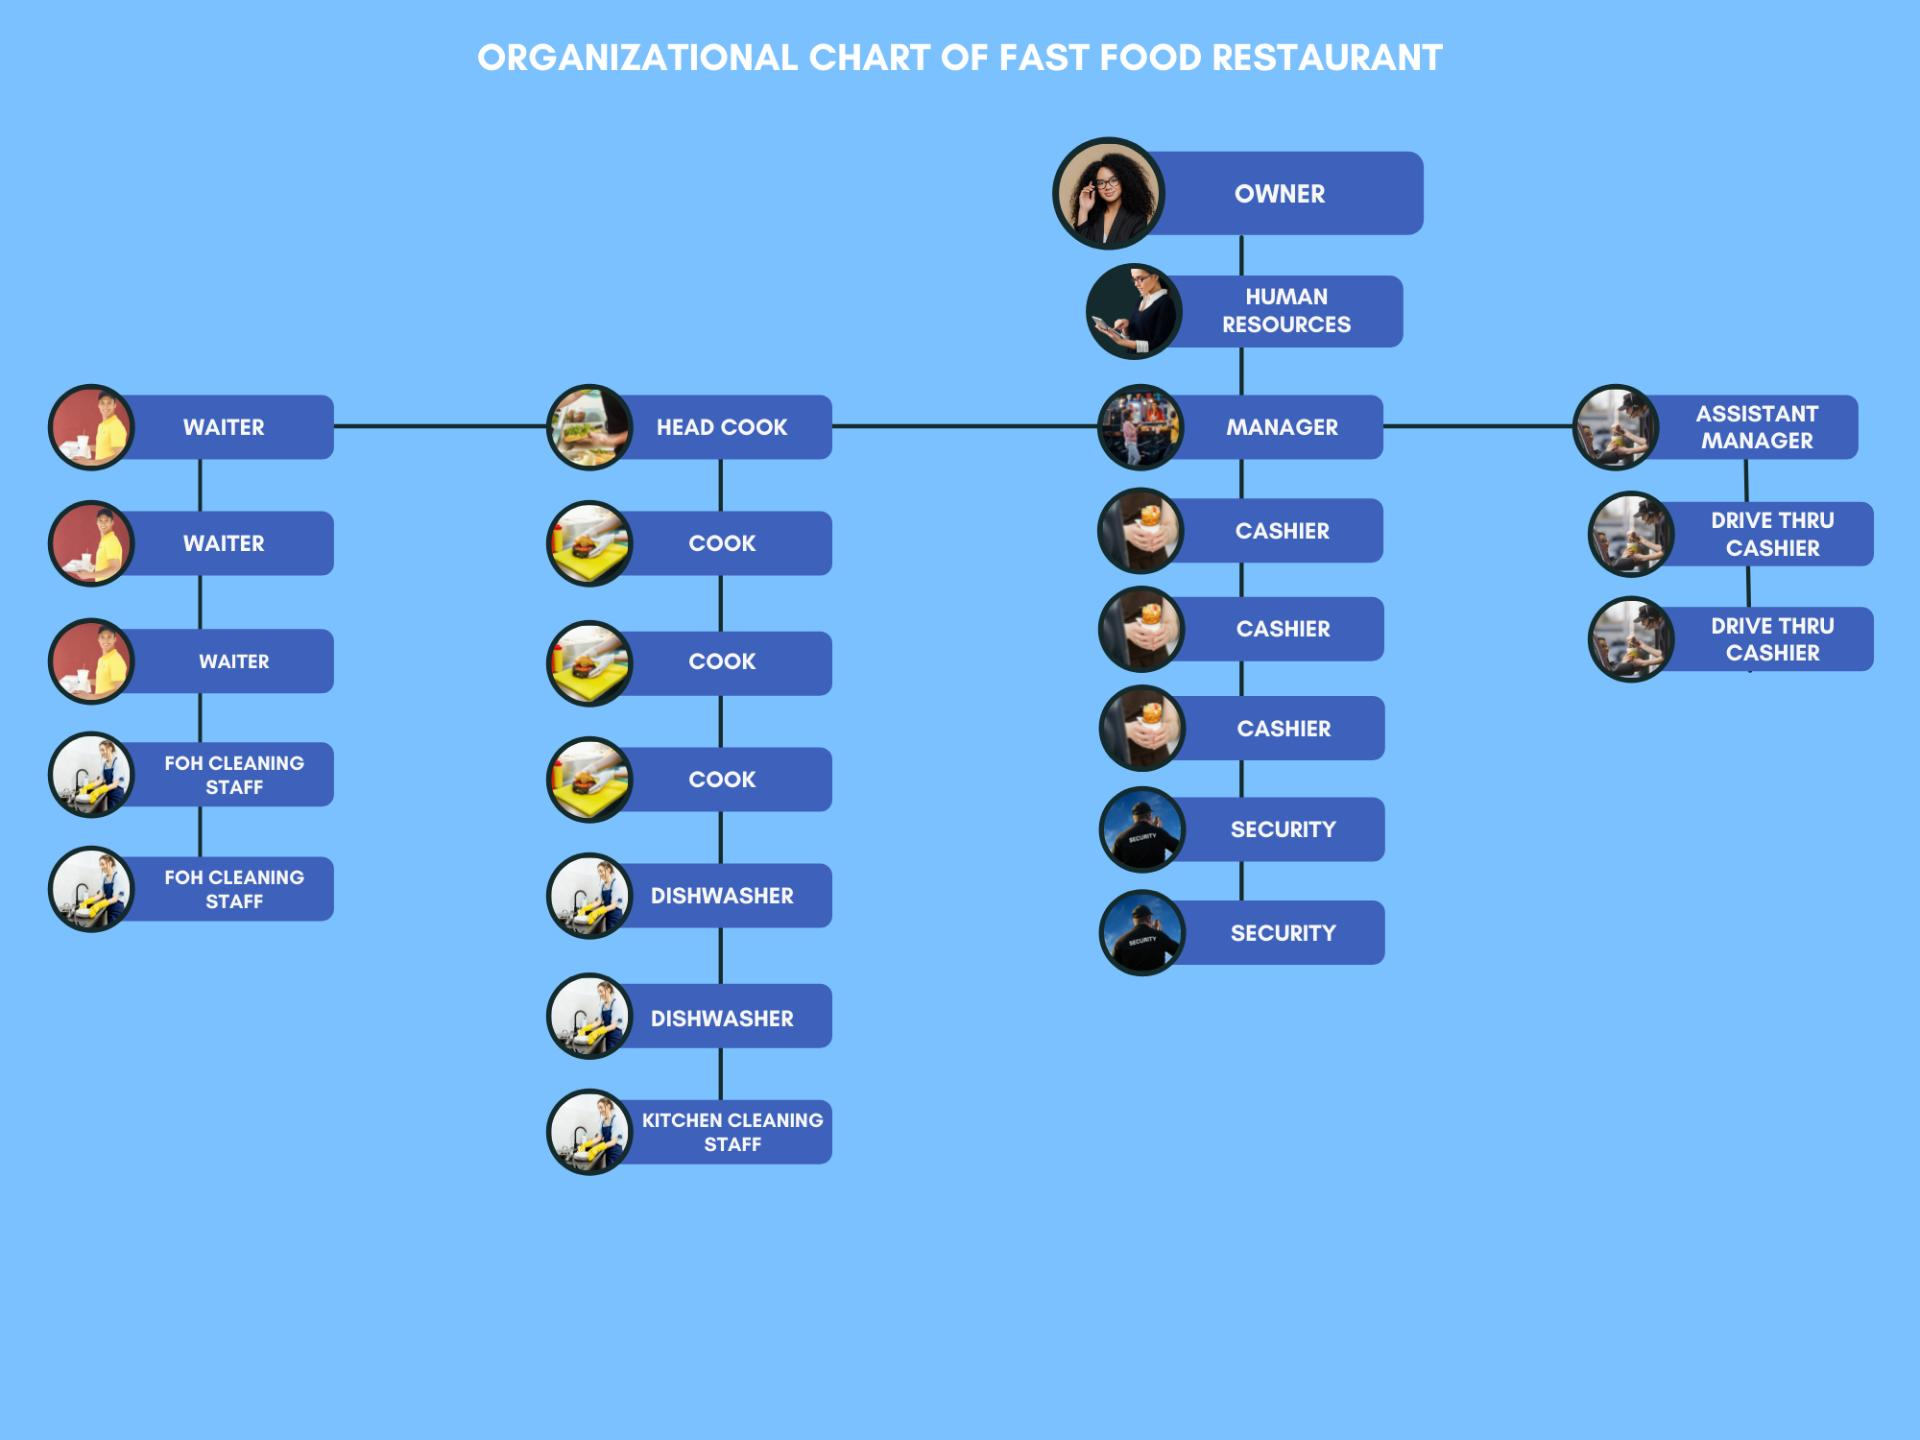
\includegraphics[width=15cm]{Images/fast-food-org-chart.jpg}
    \vspace{0.5cm}
    \caption{Sơ đồ tổ chức cho nhà hàng phục vụ đồ ăn nhanh. Nguồn: waiterio.com}
\end{figure}


\subsubsection{Sự khác nhau giữa nhà hàng ăn uống cao cấp và nhà hàng phục vụ đồ ăn nhanh}

% \begin{figure}[H]
%     \centering
%     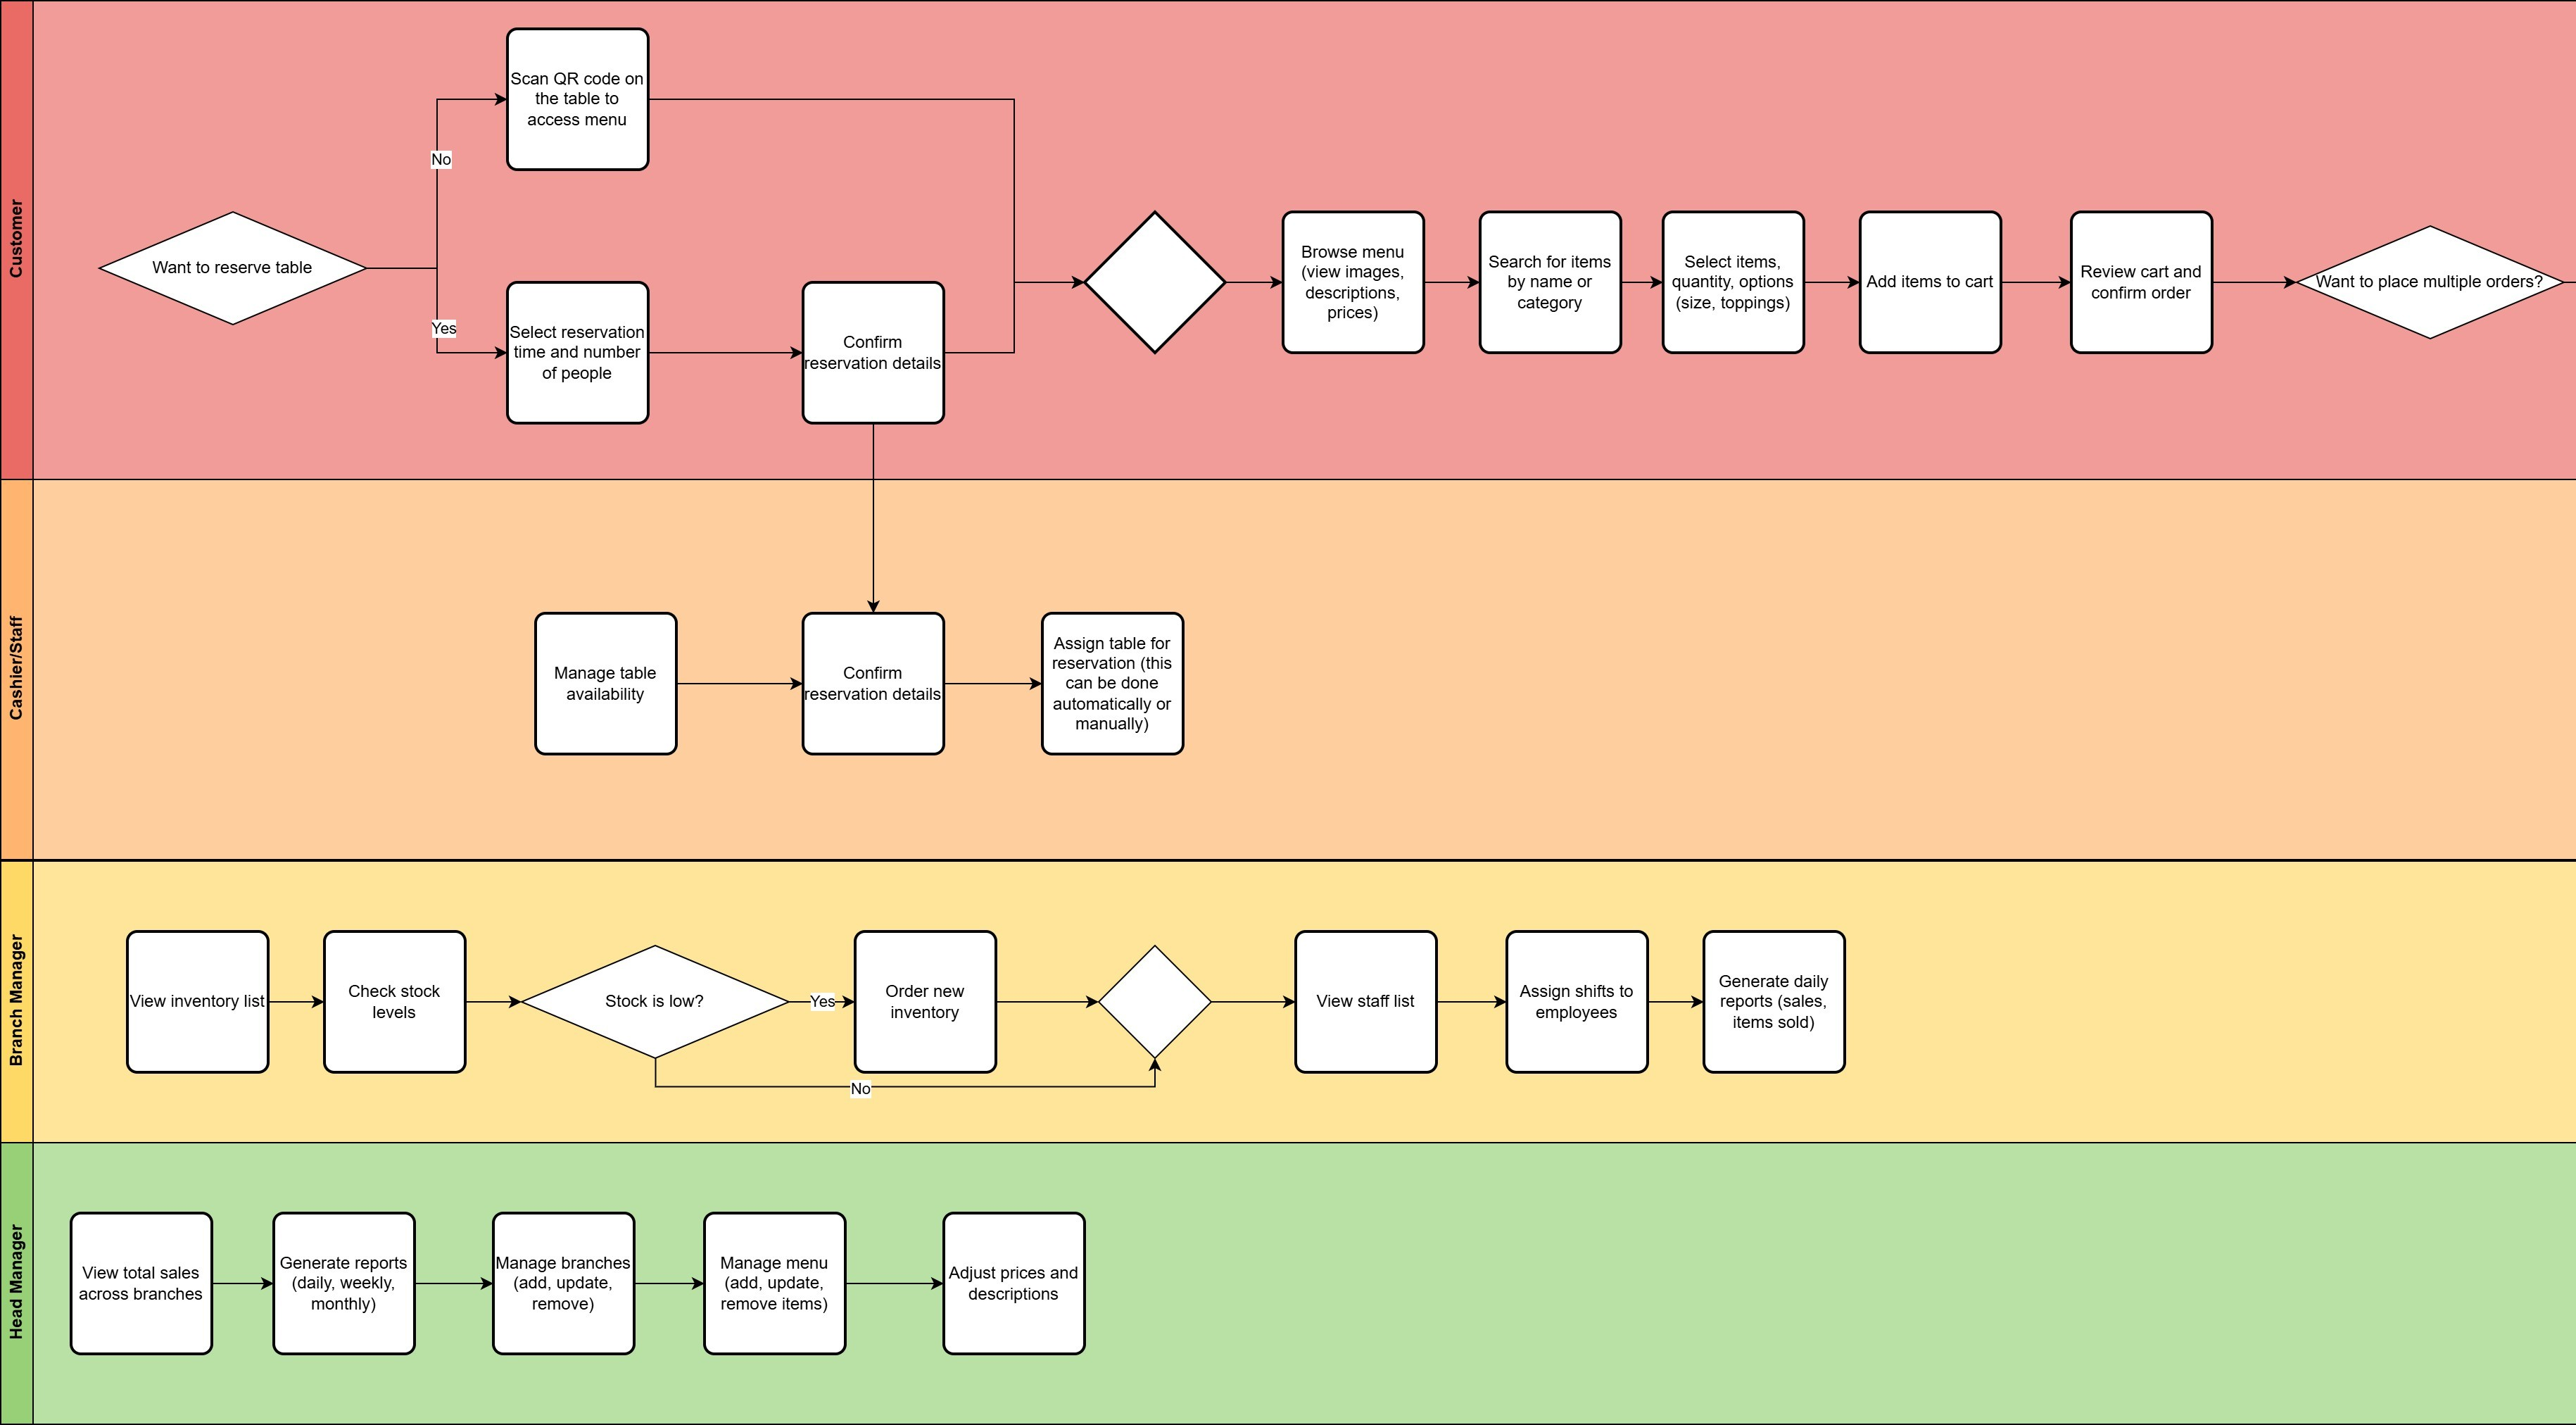
\includegraphics[width=15cm]{Images/process_map_1.jpg}
%     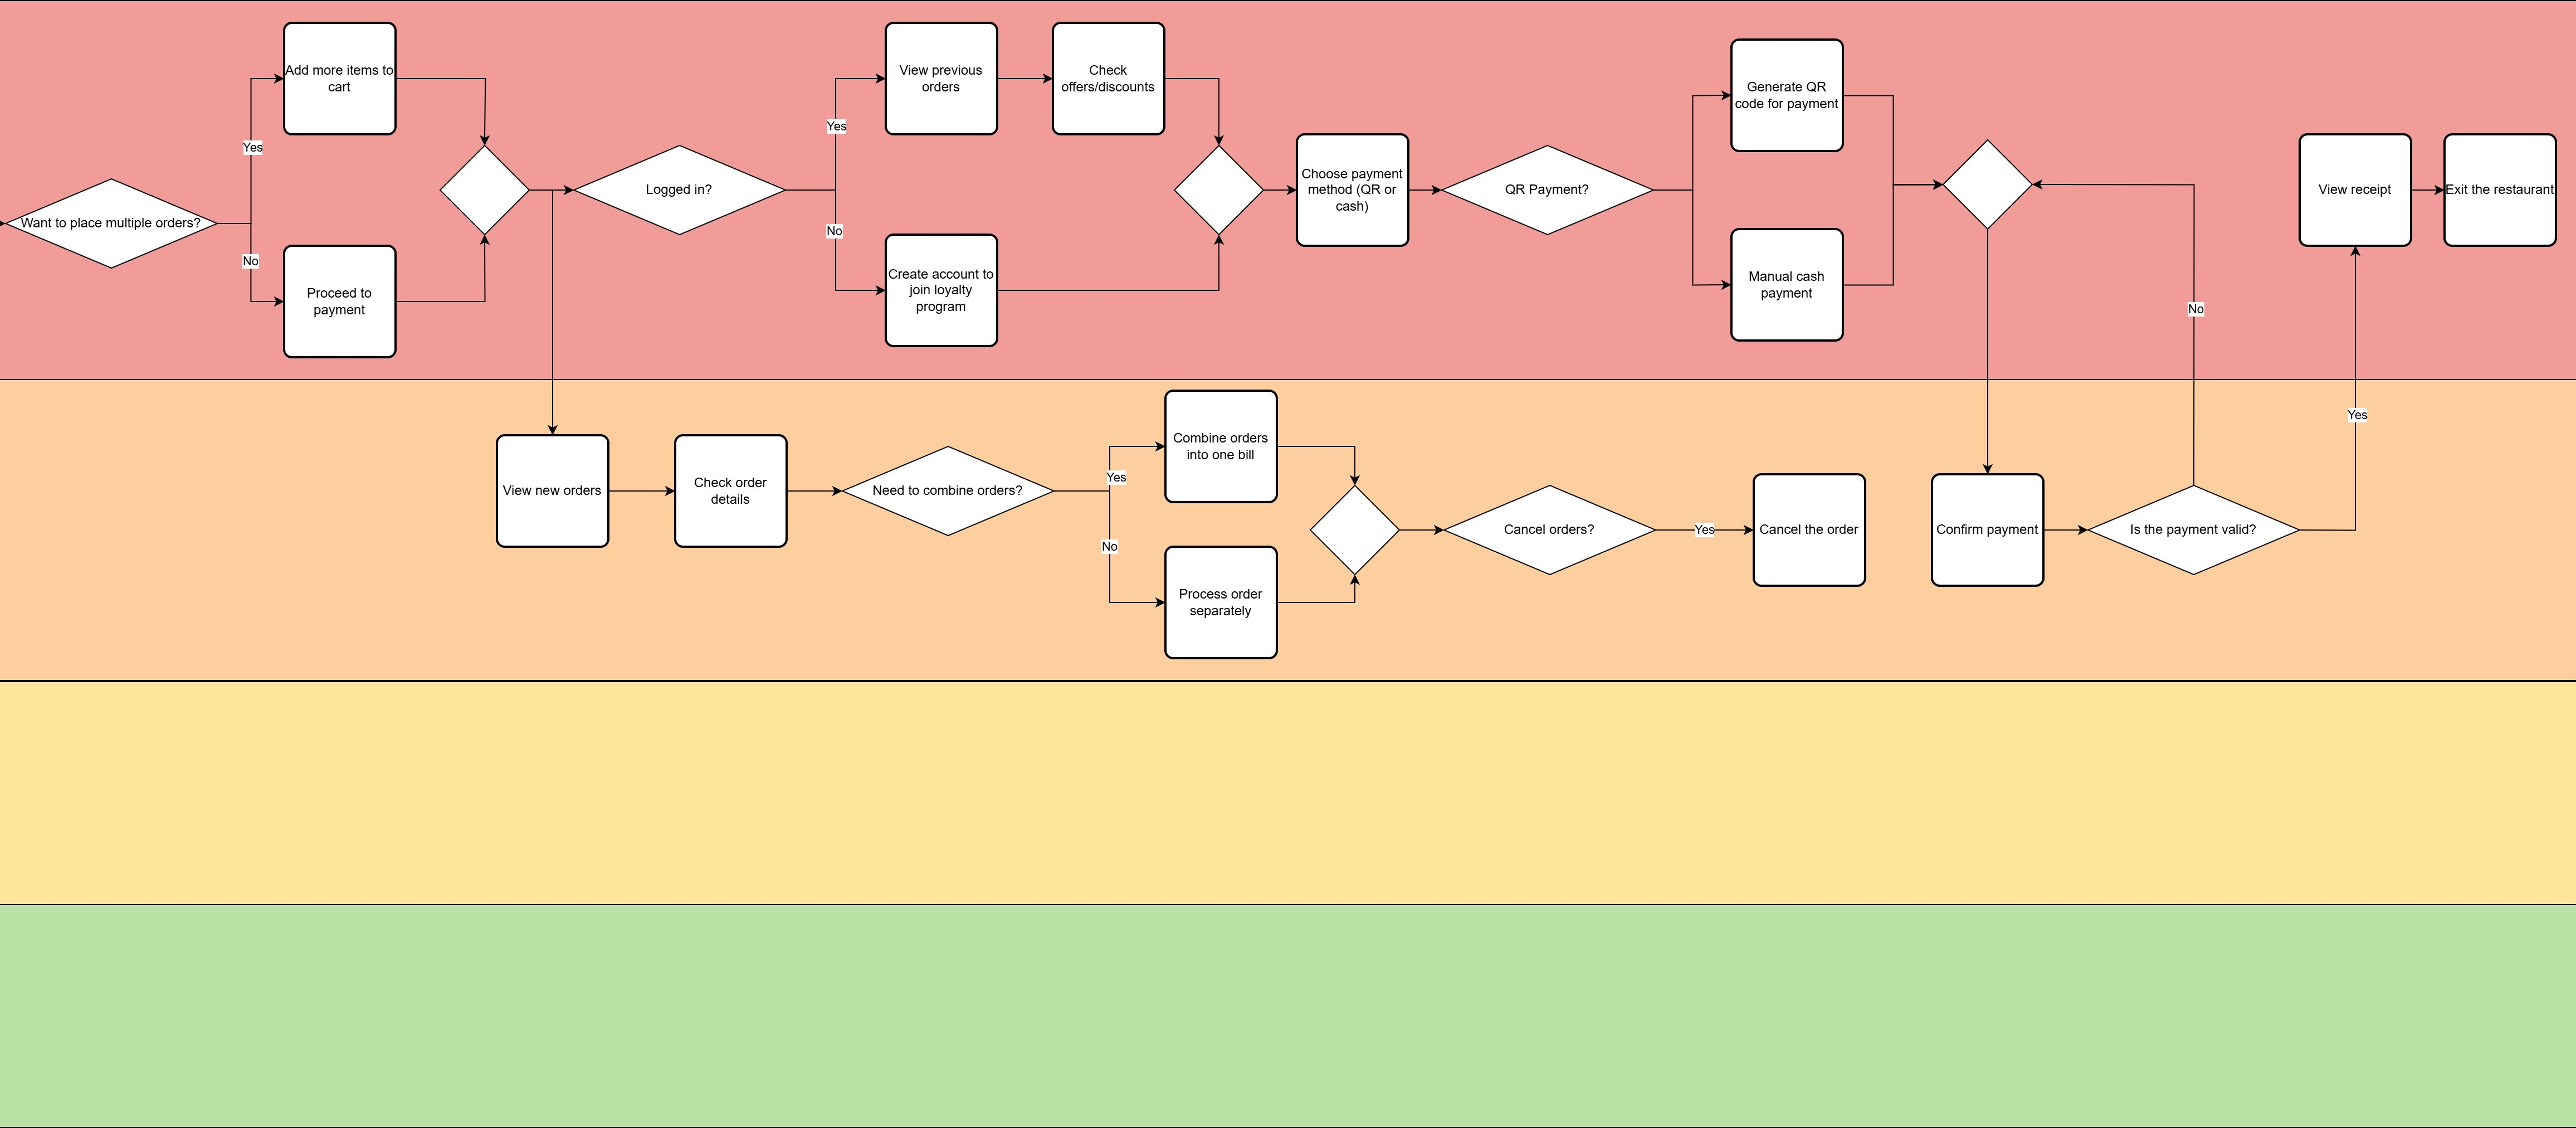
\includegraphics[width=15cm]{Images/process_map_2.jpg}
%     \vspace{0.5cm}
%     \caption{Process map về Restaurant Industry}
%     \label{fig:my_label}
% \end{figure}



\subsection*{Bảng so sánh tổng quan}

% *** THAY ĐỔI: Bắt đầu môi trường longtable ***
% Bỏ \begin{table}[H], \centering, và \resizebox
% Sử dụng p{} hoặc m{} cho các cột. p{} căn lề trên, m{} căn giữa dọc.
% Có thể dùng \RaggedRight trong các cột p/m để tránh giãn chữ không đẹp.
\begin{longtable}{| m{3.5cm} | >{\RaggedRight}m{6.5cm} | >{\RaggedRight}m{6.5cm} |} % Điều chỉnh lại chiều rộng nếu cần

% *** THAY ĐỔI: Định nghĩa Header cho bảng ***
\hline
\textbf{Tiêu chí} & \textbf{Nhà hàng Fine Dining} & \textbf{Nhà hàng Fast Food (QSR)} \\
\hline
\endfirsthead % Header chỉ xuất hiện ở đầu bảng (trang đầu tiên)

\multicolumn{3}{c}%
{{\tablename\ \thetable{} Bảng so sánh giữa nhà hàng phục vụ đồ ăn cao cấp và nhà hàng phục vụ đồ ăn nhanh}} \\ % Chú thích bảng tiếp tục
\hline
\textbf{Tiêu chí} & \textbf{Nhà hàng Fine Dining} & \textbf{Nhà hàng Fast Food (QSR)} \\
\hline
\endhead % Header lặp lại ở các trang tiếp theo

\hline \multicolumn{3}{r}{{Tiếp tục ở trang dưới}} \\ % Chú thích còn tiếp ở cuối trang (trừ trang cuối)
\endfoot

\hline % Đường kẻ cuối cùng của bảng
\endlastfoot

% *** Nội dung bảng giữ nguyên ***
\textbf{Định nghĩa \& Khái niệm} & Trải nghiệm nhà hàng tinh tế, thường đắt đỏ, đặc biệt hơn nhà hàng thông thường. Tập trung vào chất lượng cao và dịch vụ hoàn hảo. & Cơ sở cung cấp thức ăn được chuẩn bị và phục vụ nhanh chóng, thực đơn hạn chế, thường dùng đồ một lần. Tập trung vào tốc độ và sự tiện lợi. \\
\hline
\textbf{Trải nghiệm Khách hàng} & \begin{itemize} \item Sang trọng, độc quyền \item Dịch vụ cá nhân hóa, chu đáo tại bàn \item Không gian tinh tế, yên tĩnh \item Chú trọng từng chi tiết nhỏ \end{itemize} & \begin{itemize} \item Nhanh chóng, tiện lợi \item Tự phục vụ hoặc đặt tại quầy/drive-thru \item Không gian chức năng, đôi khi ồn ào \item Ít chú trọng chi tiết trải nghiệm không gian \end{itemize} \\
\hline
\textbf{Thực đơn} & \begin{itemize} \item Sáng tạo, phức tạp \item Nguyên liệu cao cấp, tươi ngon \item Thường có thực đơn cố định (set menu) hoặc gọi món (à la carte) phong phú \item Chịu ảnh hưởng lớn từ Bếp trưởng \end{itemize} & \begin{itemize} \item Hạn chế, chuẩn hóa \item Nguyên liệu tập trung vào chi phí và tốc độ chế biến \item Thường là các món phổ biến (burger, gà rán, pizza, khoai tây chiên) \item Đồng nhất giữa các chi nhánh (nếu là chuỗi) \end{itemize} \\
\hline
\textbf{Giá cả} & Cao cấp, phản ánh chất lượng nguyên liệu, kỹ năng chế biến, dịch vụ và không gian. & Thấp, phù hợp với đại chúng, tập trung vào việc bán số lượng lớn. \\
\hline
\textbf{Dịch vụ} & \begin{itemize} \item Dịch vụ tại bàn bởi nhân viên được đào tạo bài bản (waiters) \item Có Maitre d' chào đón và xếp chỗ \item Thường có Chuyên viên rượu (Sommelier) \item Tỷ lệ nhân viên/khách hàng cao \end{itemize} & \begin{itemize} \item Tự phục vụ hoặc dịch vụ tại quầy/drive-thru \item Nhân viên thực hiện các tác vụ nhanh gọn (nhận order, thu tiền, giao đồ ăn) \item Ít tương tác cá nhân hóa \item Tỷ lệ nhân viên/khách hàng thấp \end{itemize} \\
\hline
\textbf{Không gian \& Thiết kế} & Sang trọng, đầu tư vào nội thất, ánh sáng, âm nhạc, bộ đồ ăn. Thường dùng khăn trải bàn trắng. & Chức năng, hiệu quả, dễ lau dọn. Thiết kế thường theo chuẩn thương hiệu (nếu là chuỗi). Ít chú trọng yếu tố sang trọng. \\
\hline
\textbf{Mô hình Kinh doanh} & \begin{itemize} \item Chi phí vận hành rất cao (nguyên liệu, nhân sự tay nghề cao, mặt bằng đắc địa) \item Biên lợi nhuận có thể cao trên từng món nhưng tổng thể lợi nhuận là thách thức \item Phụ thuộc vào danh tiếng, đánh giá (sao Michelin), khách hàng trung thành \end{itemize} & \begin{itemize} \item Chi phí vận hành thấp hơn trên từng đơn vị sản phẩm \item Biên lợi nhuận thấp trên từng món, dựa vào bán số lượng cực lớn \item Thường hoạt động theo mô hình chuỗi, nhượng quyền (franchise) \item Marketing và nhận diện thương hiệu mạnh \end{itemize} \\
\hline
\textbf{Hoạt động Vận hành} & \begin{itemize} \item Quy trình chuẩn bị món ăn phức tạp, đòi hỏi kỹ năng cao \item Chú trọng kiểm soát chất lượng từng đĩa ăn \item Quản lý tồn kho nguyên liệu cao cấp phức tạp \end{itemize} & \begin{itemize} \item Quy trình tinh giản, dây chuyền hóa \item Sử dụng công nghệ (POS, KDS) để tối ưu tốc độ \item Chuỗi cung ứng tập trung, hiệu quả \item Đào tạo nhân viên tập trung vào tốc độ, chính xác \end{itemize} \\
\hline
\textbf{Nhân sự \& Cấu trúc Tổ chức} & \begin{itemize} \item Đội ngũ lớn, nhiều vị trí chuyên môn hóa cao (Bếp trưởng, Bếp phó, Đầu bếp chuyên khoa, Maitre d', Sommelier, Quản lý) \item Cấu trúc tổ chức phức tạp, đa tầng \item Yêu cầu kỹ năng và kinh nghiệm cao \end{itemize} & \begin{itemize} \item Đội ngũ tinh gọn hơn, các vai trò ít chuyên môn hóa hơn (Quản lý ca, Thu ngân, Nhân viên bếp, Nhân viên vệ sinh) \item Cấu trúc tổ chức phẳng, đơn giản \item Đào tạo tập trung vào quy trình chuẩn, dễ thay thế \end{itemize} \\
\hline
\textbf{Mục tiêu chính} & Cung cấp trải nghiệm ẩm thực đỉnh cao, độc đáo, xây dựng danh tiếng và thương hiệu đẳng cấp. & Tối đa hóa tốc độ phục vụ, sự tiện lợi, khối lượng bán và lợi nhuận thông qua hiệu quả vận hành. \\
% *** THAY ĐỔI: Bỏ \hline ở cuối vì \endlastfoot đã có ***
\hline % Bỏ dòng này

% *** THAY ĐỔI: Kết thúc môi trường longtable ***
% *** THAY ĐỔI: Caption và label đặt BÊN TRONG longtable ***
\caption{Bảng so sánh giữa nhà hàng phục vụ đồ ăn cao cấp và nhà hàng phục vụ đồ ăn nhanh}
\label{tab:comparison_detail} \\
\end{longtable}


Sự tương phản giữa nhà hàng fine dining và fast food không chỉ dừng lại ở các yếu tố bề mặt như giá cả hay tốc độ. Nó bắt nguồn từ triết lý kinh doanh, đối tượng khách hàng mục tiêu, và mô hình vận hành hoàn toàn khác biệt, dẫn đến những hệ quả sâu sắc:

\begin{itemize}
    \item \textbf{Giá trị cốt lõi:} Fine dining bán một \textit{trải nghiệm toàn diện}, nơi ẩm thực chỉ là một phần (dù là phần quan trọng nhất). Các yếu tố như không gian, dịch vụ cá nhân hóa, sự độc quyền, và cảm giác được chăm sóc đặc biệt đóng góp lớn vào giá trị mà khách hàng nhận được và sẵn sàng chi trả cao. Ngược lại, fast food bán \textit{sự tiện lợi và tính nhất quán}. Khách hàng tìm đến vì tốc độ, giá cả phải chăng và biết chính xác họ sẽ nhận được gì ở bất kỳ chi nhánh nào của thương hiệu.

    \item \textbf{Rủi ro và Lợi nhuận:} Mô hình fine dining có rủi ro cao hơn do chi phí đầu tư và vận hành lớn, cùng sự phụ thuộc vào danh tiếng và lượng khách hàng giới hạn. Một đánh giá tiêu cực hoặc thay đổi xu hướng ẩm thực có thể ảnh hưởng nghiêm trọng. Tuy nhiên, khi thành công, biên lợi nhuận trên mỗi khách hàng có thể rất cao. Fast food có rủi ro thấp hơn trên từng giao dịch nhờ mô hình chuẩn hóa và khối lượng lớn. Lợi nhuận đến từ việc tối ưu hóa chi phí và quy mô, nhưng lại nhạy cảm với cạnh tranh về giá và chi phí nguyên liệu đầu vào.

    \item \textbf{Vai trò của Con người và Công nghệ:} Trong fine dining, yếu tố con người là không thể thay thế. Kỹ năng của đầu bếp, sự tinh tế của nhân viên phục vụ, và kiến thức của sommelier tạo nên sự khác biệt. Công nghệ chủ yếu hỗ trợ quản lý (đặt bàn, POS) chứ không thay thế vai trò trung tâm của con người trong việc tạo ra trải nghiệm. Ngược lại, fast food tận dụng tối đa công nghệ để \textit{tăng hiệu suất và giảm sự phụ thuộc vào kỹ năng cá nhân}. Từ hệ thống đặt hàng tự động, bếp dây chuyền, đến phân tích dữ liệu bán hàng, công nghệ là chìa khóa để duy trì tốc độ và sự đồng nhất.

    \item \textbf{Cấu trúc tổ chức phản ánh sự phức tạp:} Sơ đồ tổ chức đa tầng của fine dining cho thấy sự chuyên môn hóa cao độ cần thiết để duy trì chất lượng ở mọi khâu, từ bếp đến tiền sảnh. Mỗi vị trí có vai trò và trách nhiệm rõ ràng, đòi hỏi kỹ năng chuyên biệt. Cấu trúc phẳng của fast food phản ánh quy trình làm việc đơn giản, lặp lại và tập trung vào hiệu quả hoạt động theo ca dưới sự giám sát của quản lý ca.

    \item \textbf{Thích ứng và Xu hướng:} Cả hai mô hình đều đang phải thích ứng. Fine dining ngày càng chú trọng hơn đến tính bền vững, nguồn gốc nguyên liệu và trải nghiệm độc đáo (ví dụ: bếp mở, tương tác với đầu bếp). Một số nhà hàng fine dining cũng tìm cách tiếp cận phân khúc rộng hơn thông qua các mô hình "casual dining" hoặc "bistro" cao cấp. Fast food đang đối mặt với áp lực về thực phẩm lành mạnh hơn, nguồn gốc rõ ràng và trải nghiệm khách hàng tốt hơn (không gian sạch đẹp, dịch vụ thân thiện hơn). Sự trỗi dậy của "fast-casual" (phân khúc giữa fast food và casual dining) là minh chứng cho sự thay đổi này, kết hợp tốc độ của fast food với chất lượng nguyên liệu và không gian tốt hơn.

\end{itemize}

\subsection{Hành trình khách hàng (Customer Journey) trong ngành dịch vụ nhà hàng}

Hành trình khách hàng trong ngành dịch vụ nhà hàng là một chuỗi các tương tác và trải nghiệm, từ giai đoạn nhận thức ban đầu đến hành động quay lại sử dụng dịch vụ. Hiểu rõ và tối ưu hóa từng giai đoạn trong hành trình này là yếu tố then chốt để nâng cao sự hài lòng của khách hàng, xây dựng lòng trung thành và tạo lợi thế cạnh tranh bền vững cho nhà hàng. Theo Orderable \cite{Orderable}, hành trình khách hàng trong ngành dịch vụ nhà hàng có thể chia thành các cột mốc như sau:

\begin{figure}[H]
    \centering
    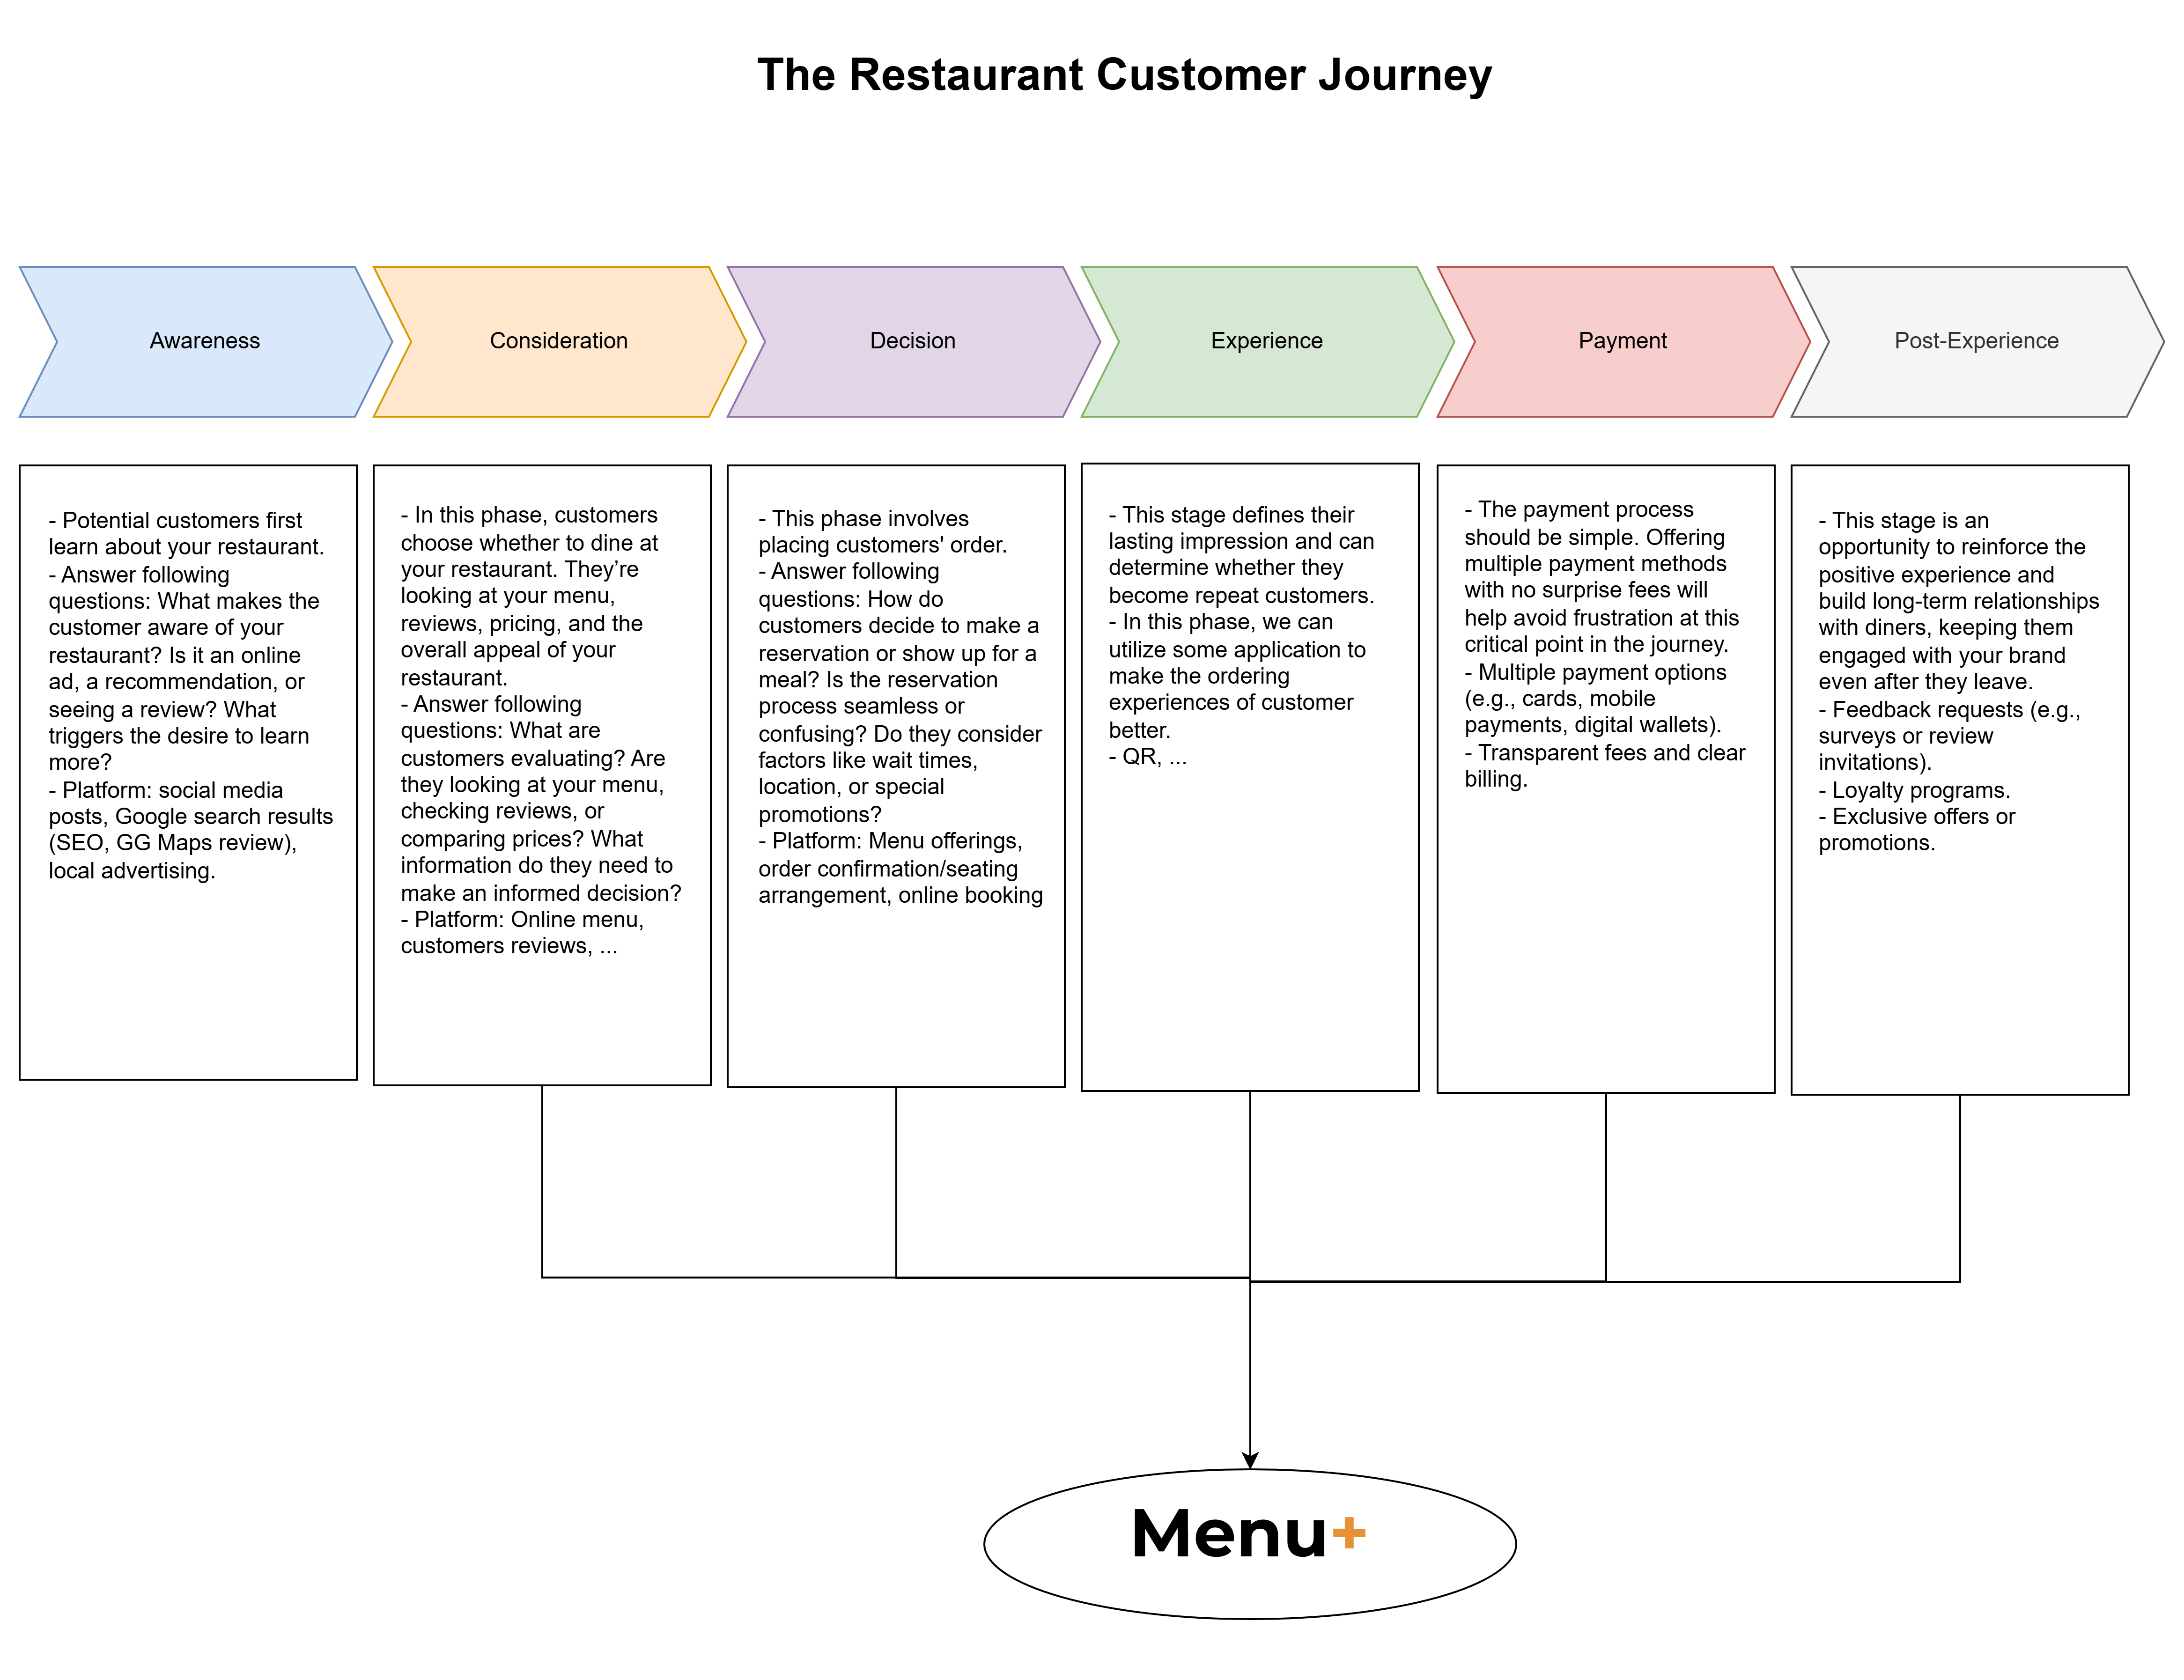
\includegraphics[width=15cm]{Images/restaurant-customer-journey.png}
    \caption{Giới thiệu về Hành trình Khách hàng trong Nhà hàng.}
    \label{fig:my_label}
\end{figure}

\begin{enumerate}
    \item Giai đoạn Nhận thức (Awareness): Giai đoạn này đánh dấu điểm tiếp xúc đầu tiên của khách hàng tiềm năng với nhà hàng. Các kênh truyền thông đa dạng, từ quảng cáo trực tuyến (ví dụ: Google Ads, quảng cáo trên mạng xã hội), đánh giá trực tuyến (ví dụ: Google Reviews, TripAdvisor), đến các phương pháp truyền thống như quảng cáo in ấn, giới thiệu từ người thân, đóng vai trò quan trọng trong việc tạo dựng nhận diện thương hiệu.
    \item Giai đoạn Cân nhắc (Consideration): Sau khi nhận biết về nhà hàng, khách hàng tiềm năng sẽ tiến hành thu thập thông tin chi tiết hơn, so sánh với các lựa chọn khác. Họ sẽ xem xét thực đơn, bảng giá, hình ảnh không gian, đọc các đánh giá chi tiết và có thể tham khảo ý kiến từ bạn bè, người thân.
    \item Giai đoạn Quyết định (Decision): Giai đoạn này là thời điểm khách hàng đưa ra quyết định lựa chọn nhà hàng. Các yếu tố ảnh hưởng đến quyết định bao gồm sự thuận tiện trong việc đặt bàn, vị trí địa lý, đánh giá tổng quan về nhà hàng, và các chương trình khuyến mãi, ưu đãi đặc biệt.
    \item Giai đoạn Trải nghiệm (Experience): Đây là giai đoạn quan trọng nhất, khi khách hàng trực tiếp trải nghiệm dịch vụ và sản phẩm tại nhà hàng. Chất lượng món ăn, thái độ phục vụ, không gian nhà hàng, sự sạch sẽ và tiện nghi đều đóng vai trò then chốt. Việc ứng dụng công nghệ, ví dụ như hệ thống gọi món, thanh toán không tiền mặt, có thể nâng cao trải nghiệm khách hàng.
    \item Giai đoạn Thanh toán (Payment): Quá trình thanh toán cần được thực hiện nhanh chóng, chính xác và thuận tiện. Cung cấp đa dạng các phương thức thanh toán (ví dụ: tiền mặt, thẻ tín dụng, ví điện tử) để đáp ứng nhu cầu của khách hàng.
    \item Giai đoạn Hậu trải nghiệm (Post-Experience): Sau khi khách hàng rời nhà hàng, việc duy trì kết nối và khuyến khích quay lại là rất quan trọng. Gửi email cảm ơn, mời tham gia khảo sát đánh giá, cung cấp các chương trình khách hàng thân thiết, và gửi các ưu đãi đặc biệt là những phương pháp hiệu quả.
\end{enumerate}

\subsection{Mô hình MVC}
MVC là viết tắt của khái niệm "Model-View-Controller", một trong những mô hình thiết kế phần mềm phổ biến nhất.\\

MVC tách biệt dữ liệu, giao diện người dùng và logic xử lý thành ba thành phần riêng biệt nhưng vẫn được kết nối chặt chẽ với nhau.

\begin{itemize}
    \item Model (M): Đại diện cho dữ liệu và logic xử lý các nghiệp vụ của ứng dụng.
    \item View (V): Quản lý giao diện và hiển thị dữ liệu ra cho người dùng.
    \item Controller (C): Làm điều phối và điều hướng tương tác giữa Model và View. Nó nhận yêu cầu từ View, thực hiện xử lý trên Model và trả kết quả về cho View hiển thị.
\end{itemize}

MVC giúp tách biệt các thành phần của ứng dụng, tăng tính bảo trì và khả năng mở rộng trong tương lai \cite{MVC}.

\begin{figure}[H]
    \centering
    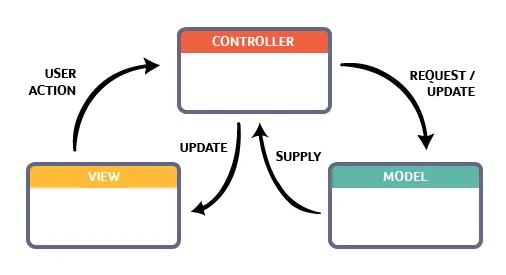
\includegraphics[width=10cm]{Images/ezgif-4-c53032b3fd.png}
    \vspace{0.5cm}
    \caption{MVC là gì?}
    \label{fig:my_label}
\end{figure}

Mô hình MVC (MVC pattern) thường được dùng để phát triển giao diện người dùng. Nó cung cấp các thành phần cơ bản để thiết kế một chương trình cho máy tính hoặc điện thoại di động, cũng như là các ứng dụng web.

\subsubsection{Các thành phần của MVC}
Mô hình MVC gồm 3 loại chính là thành phần bên trong không thể thiếu khi áp dụng mô hình này:
\begin{figure}[H]
    \centering
    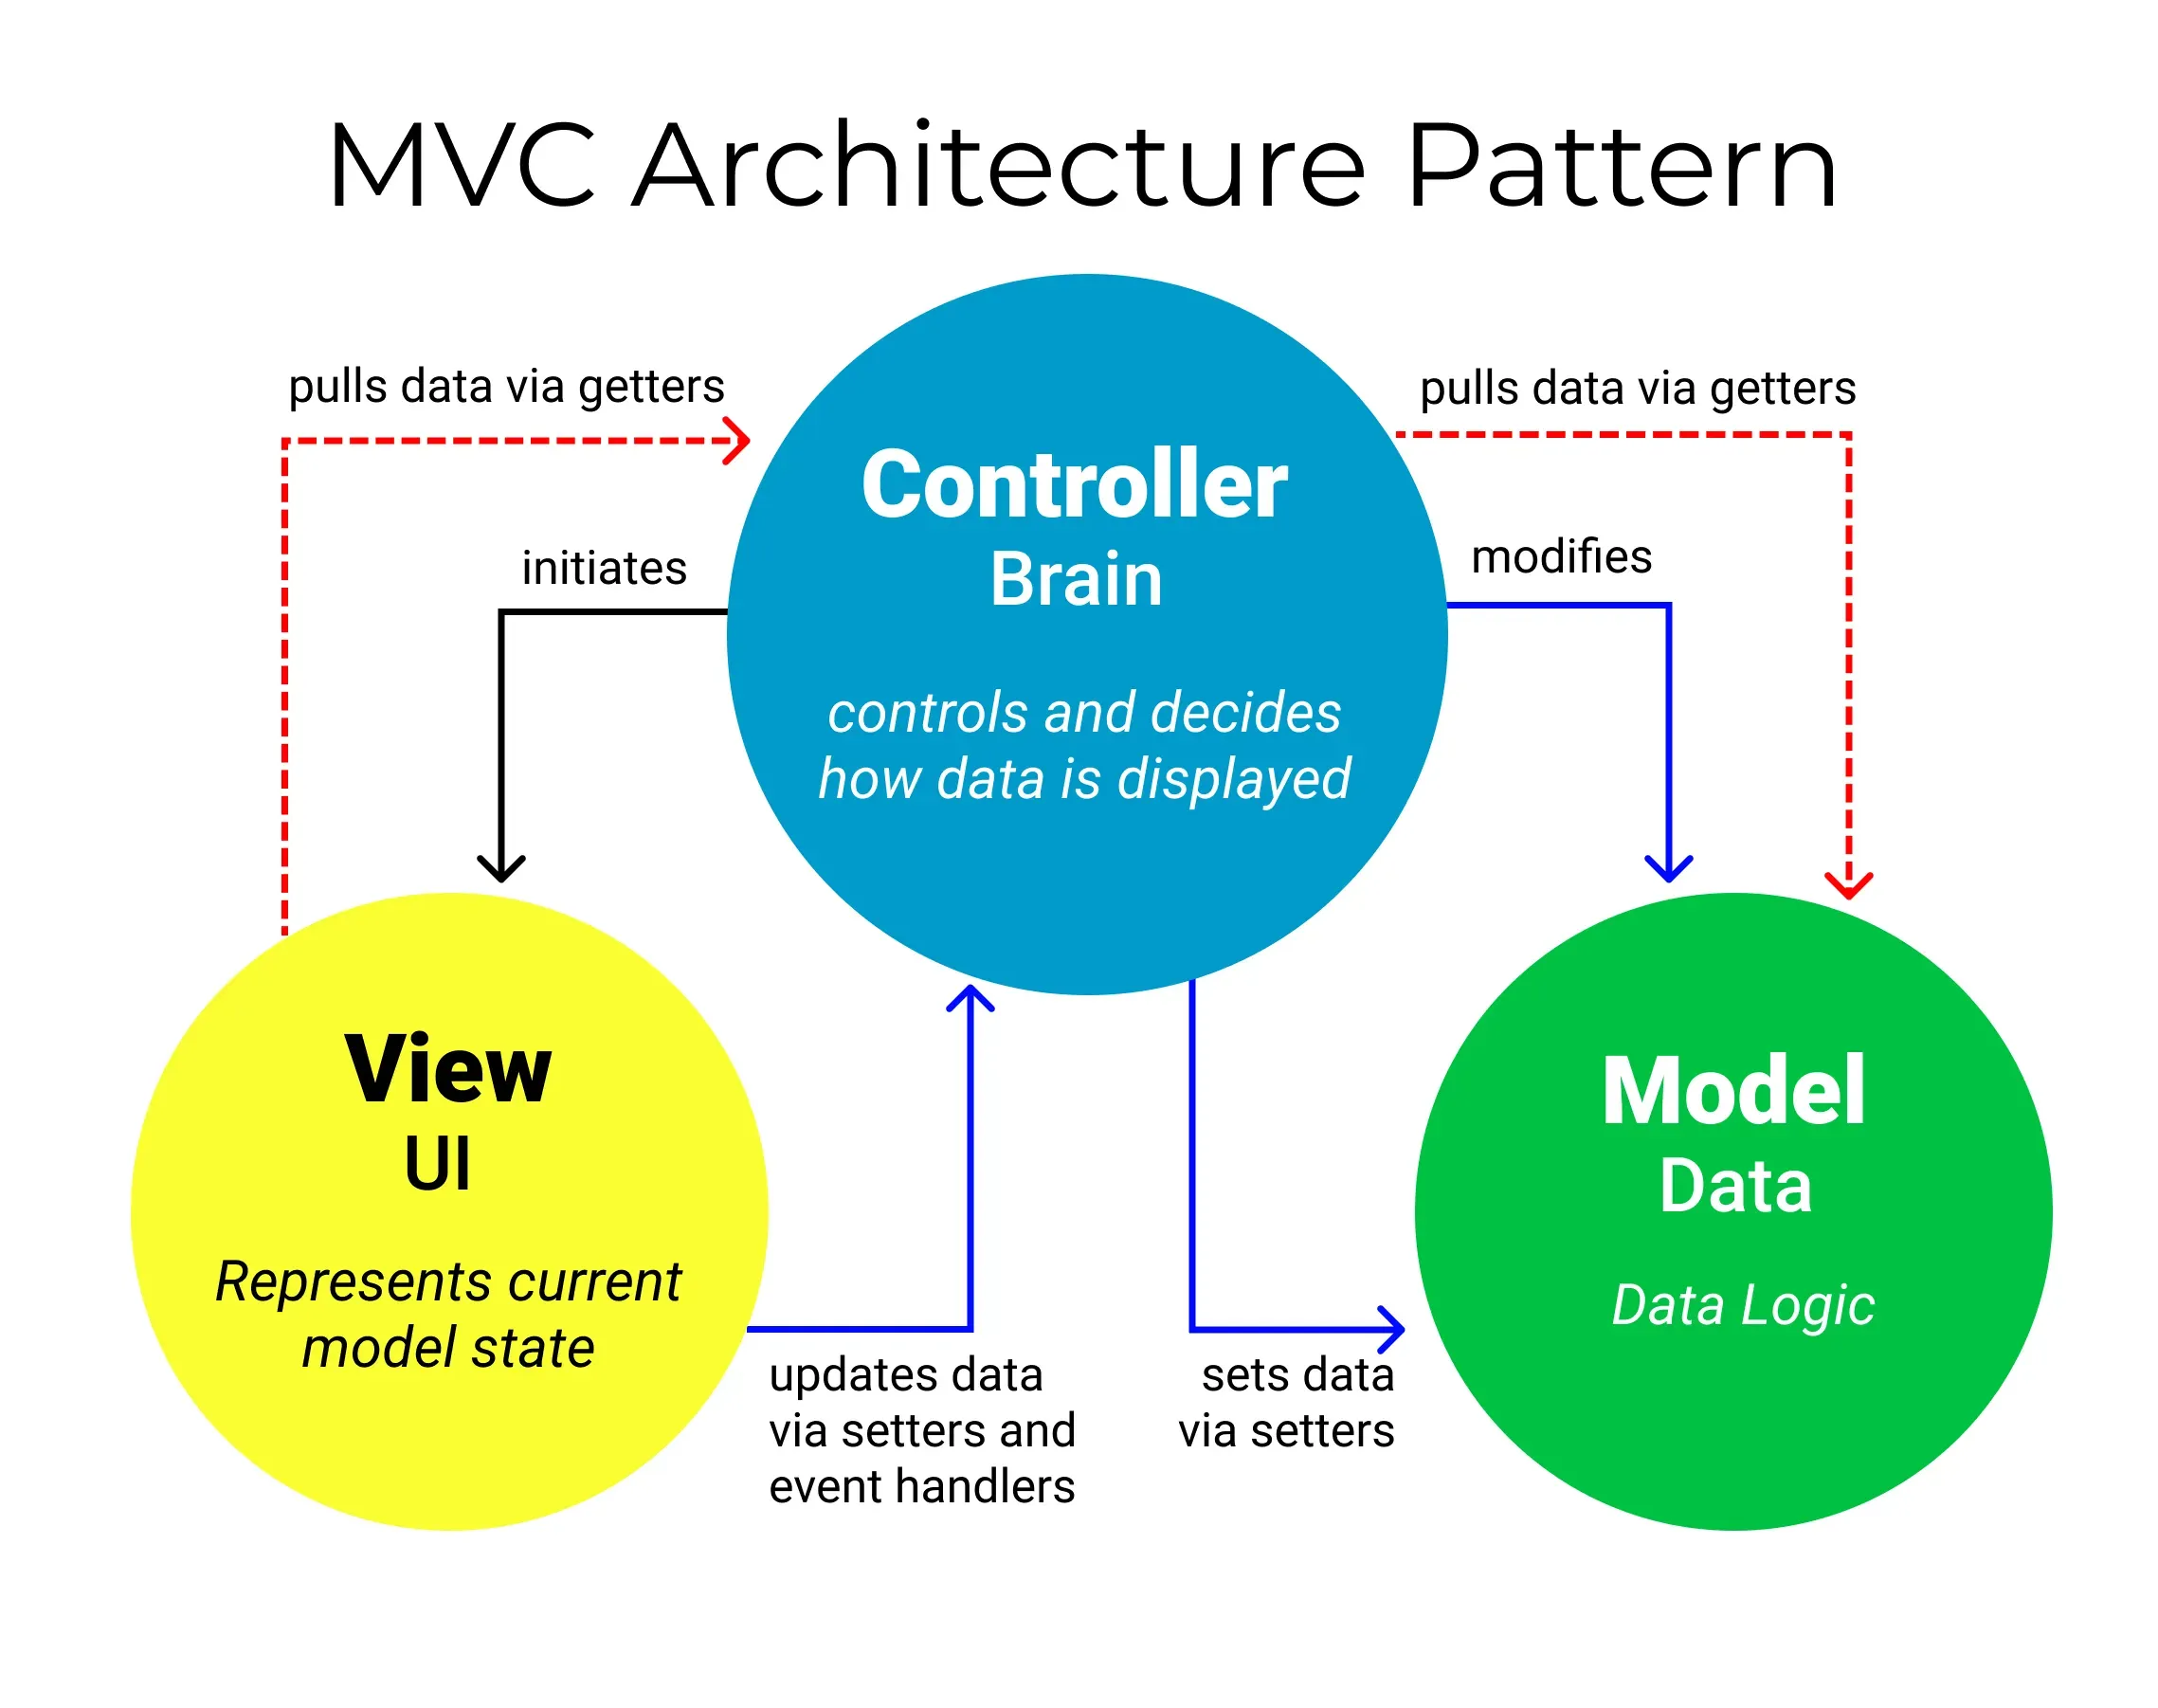
\includegraphics[width=10cm]{Images/cacthanhphanmvc.png}
    \vspace{0.5cm}
    \caption{Thành phần của MVC}
    \label{fig:my_label}
\end{figure}

\begin{itemize}
    \item Model: Là bộ phận có chức năng lưu trữ toàn bộ dữ liệu của ứng dụng và là cầu nối giữa 2 thành phần bên dưới là View và Controller. Một model là dữ liệu được sử dụng bởi chương trình. Đây có thể là cơ sở dữ liệu, hoặc file XML bình thường hay một đối tượng đơn giản. Chẳng hạn như biểu tượng hay là một nhân vật trong game.
    \item View: Đây là phần giao diện (theme) dành cho người sử dụng. View là phương tiện hiển thị các đối tượng trong một ứng dụng. Chẳng hạn như hiển thị một cửa sổ, nút hay văn bản trong một cửa sổ khác. Nó bao gồm bất cứ thứ gì mà người dùng có thể nhìn thấy được.
    \item Controller: Là bộ phận có nhiệm vụ xử lý các yêu cầu người dùng đưa đến thông qua View. Một controller bao gồm cả Model lẫn View. Nó nhận input và thực hiện các update tương ứng.
\end{itemize}

\subsubsection{Luồng xử lý trong MVC}
Luồng xử lý trong của mô hình MVC, bạn có thể hình dung cụ thể và chi tiết qua từng bước dưới đây:
\begin{itemize}
    \item Khi một yêu cầu của từ máy khách (Client) gửi đến Server. Thì bị Controller trong MVC chặn lại để xem đó là URL request hay sự kiện.
    \item Sau đó, Controller xử lý input của user rồi giao tiếp với Model trong MVC.
    \item Model chuẩn bị data và gửi lại cho Controller.
    \item Cuối cùng, khi xử lý xong yêu cầu thì Controller gửi dữ liệu trở lại View và hiển thị cho người dùng trên trình duyệt.
\end{itemize}
\begin{figure}[H]
    \centering
    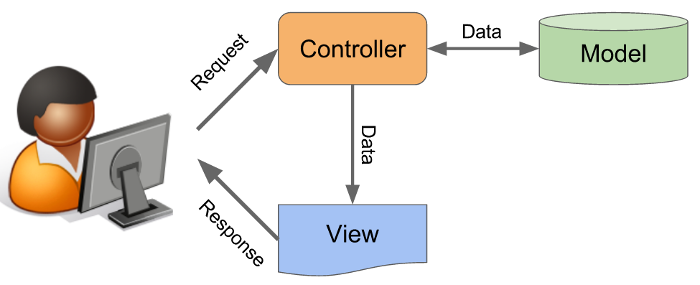
\includegraphics[width=10cm]{Images/luongmvc.png}
    \vspace{0.5cm}
    \caption{View và Model sẽ được xử lý bởi Controller}
    \label{fig:my_label}
\end{figure}

Ở đây, View không giao tiếp trực tiếp với Model. Sự tương tác giữa View và Model sẽ chỉ được xử lý bởi Controller.